\chapter{T2K and SK Experiment Overview}
\label{chap:T2KSKExp}

\finish{This needs some references!}

\section{The Super-Kamiokande Experiment}
\label{sec:T2KSKExp_SK}

The SK experiment began taking data in 1996 and has had many modifications throughout its lifespan. There has been six defined periods of data taking as noted in \autoref{tab:T2KSKExp_SKPeriods}. Between the SK-I and SK-II periods, a significant proportion of the PMTs were damaged during maintainence. Those that survived were equally distributed throughout the detector which resulted in a reduced photo-coverage. From SK-III onwards, the full suite of PMTs were operational. Before the start of SK-IV, the datta acquisition system was upgraded. Between SK-IV and SK-V, a significant effort was placed into tank open maintainence and repair/replacement of defective PMTs, a task in which the author of this thesis was required for. Consequently, the detector conditions were significantly different between the two operational periods. SK-VI saw the start of the \quickmath{0.01\%} gadonlium doped water being introduced into the tank and the detector continues to operate to this day. Efforts are currently underway to increase the gadolinium concentrate in the likely start of the next SK period.

\begin{table}[ht!]
    \centering
    \begin{tabular}{c|l|l|c}
      \hline
      Period & Start Date & End Date & Live-time (days) \\
      \hline
      I & April 1996 & July 2001 & 0 \\
      II & October 2002 & October 2005 & 0 \\
      III & July 2006 & September 2008 & 0 \\
      IV & September 2008 & May 2018 & 0 \\
      V & January 2019 & July 2020 & 0 \\
      VI & July 2020 & Ongoing & 0 \\
      \hline 
      \hline
    \end{tabular}
    \caption{The different SK periods throughout the experiments lifetime.}
    \label{tab:T2KSKExp_SKPeriods}
\end{table}

\subsection{The SK Detector}
\label{subsec:T2KSKExp_SKDetector}

The basic structure of the Super-Kamiokande (SK) detector is a cylindrical tank with diameter \quickmath{39.3\text{m}} and hieght \quickmath{41.1\text{m}} filled with ultrapure water. A diagram of the signficant parts of the SK detector is illustrated in \autoref{fig:T2KSKExp_SK_Diag}. The SK detector is situated in the Kamioka mine in Gifu, Japan. The cavern in which the detector is located is underground with roughly \quickmath{1\text{km}} rock overburden (\quickmath{2.7 \text{km}} water equivalent overburden). At this depth, the rate of cosmic ray muons is significantly decreased to a value of \quickmath{\approx 2\text{Hz}}, compared to a surface-level detector. The top of the tank is covered with stainless steel which is designed as a working platform for maintainence, calibration and location for high voltage and data acquisition electronics.

\begin{figure}[h]
  \begin{subfigure}[t]{0.95\textwidth}
    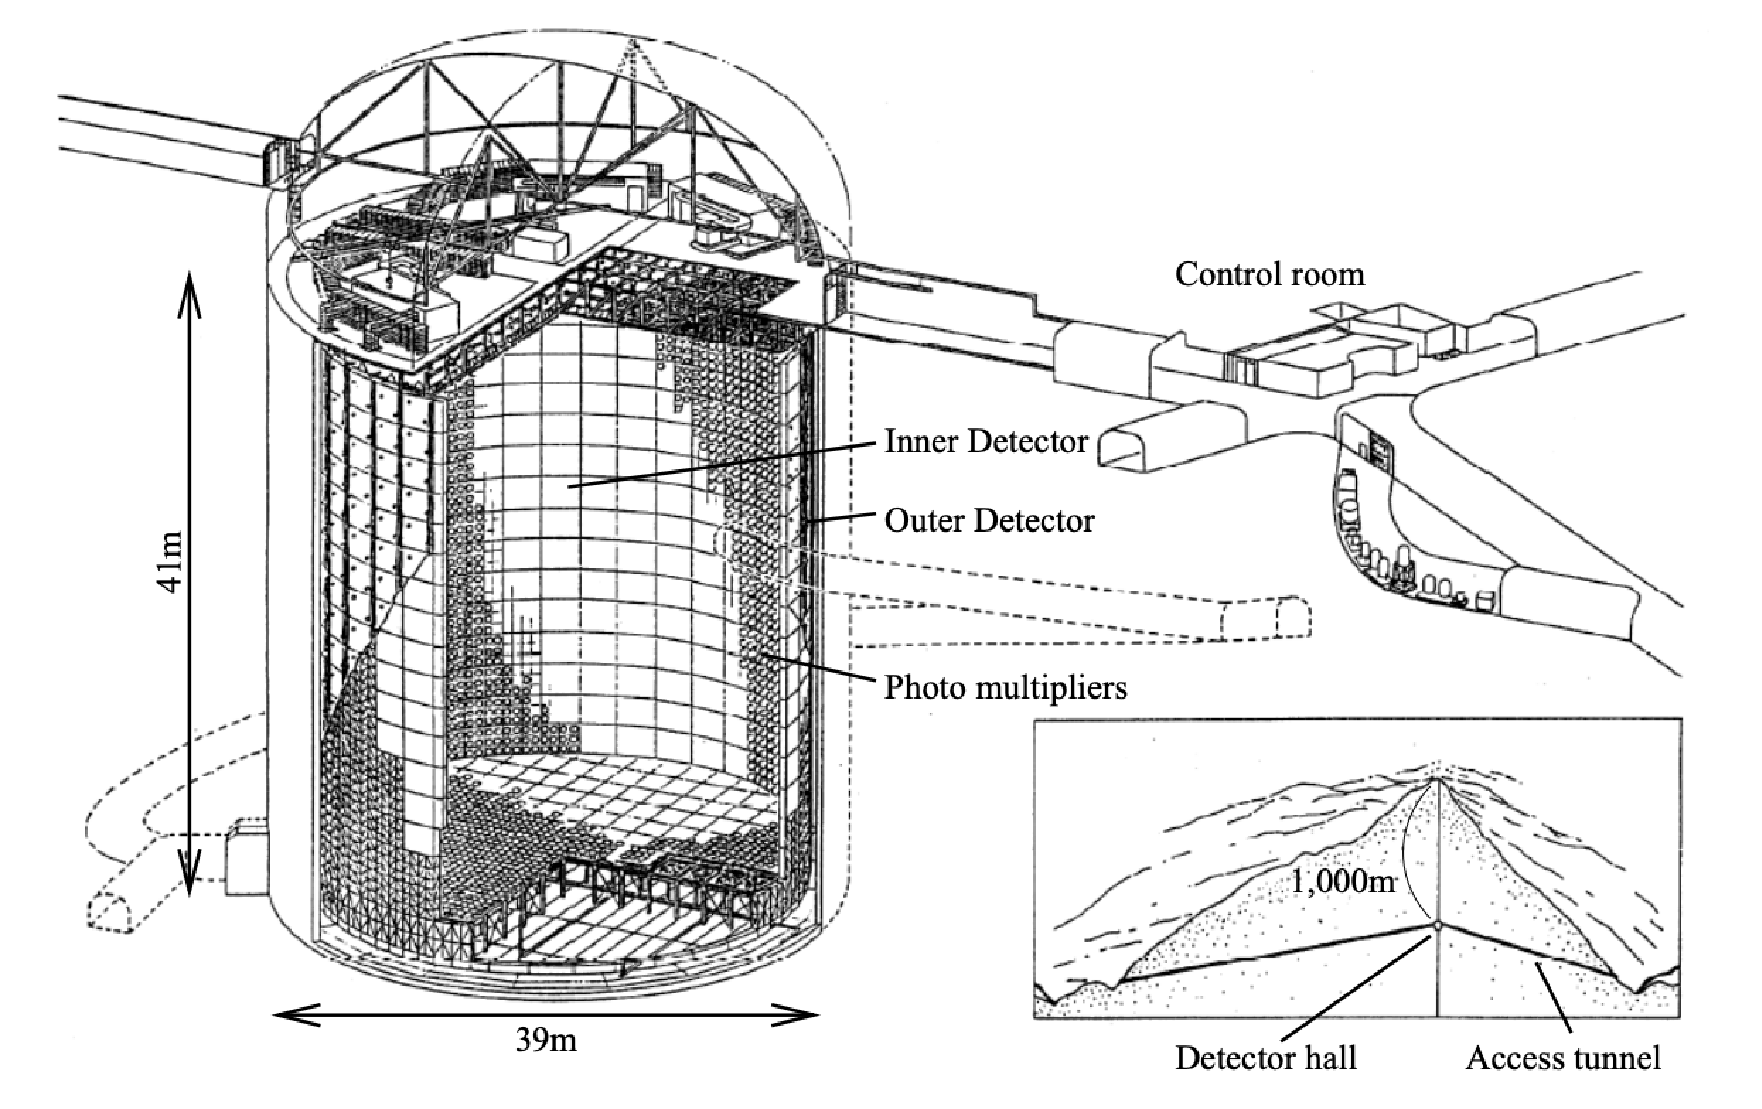
\includegraphics[width=\textwidth, trim={0mm 0mm 0mm 0mm}, clip,page=1]{Figures/Detectors/SKDiagram.pdf}
  \end{subfigure}
  \caption{A schematic diagram of the Super-Kamiokande Detector. Taken from \cite{Itow2001-bc}.}
  \label{fig:T2KSKExp_SK_Diag}
\end{figure}

A smaller cylindrical structure (\quickmath{36.2\text{m}} diameter, \quickmath{33.8\text{m}} hieght) is situated inside the tank, with an approximate \quickmath{2\text{m}} gap between this structure and the outer tank wall. The purpose of this structure is to support the photomultiplier tubes (PMTs). The volume inside and outside the support structure are referred to as the inner detector (ID) and outer detector (OD), respectively. The ID and OD are instrumented by \quickmath{11129} \quickmath{50\text{cm}} and \quickmath{1885} \quickmath{20 \text{cm}} PMTs respectively. The inner detector contains a \quickmath{32\text{kton}} volume of water, although many analyses performed at SK use a ``fiducial volume'' defined by the volume of water inside the ID excluding some distance to the ID wall. This reduces the volume of detector which is sensitive to neutrino events but reduces radioactive backgrounds and allows for better constraints on the reconstruction systematics. The nominal fiducial volume is defined as the area contained inside \quickmath{2\text{m}} from the ID wall for a total of \quickmath{22.5\text{kton}} water.

The two regions of the detector (ID and OD) are optically separated with opaque black plastic. The purpose of this is to deteremine whether a track entered or exited the ID. This allows cosmic muon rays and partially contained events to be tagged and separated from neutrino events entirely contained within the detector's sensitive region. This black plastic is also used to cover the area between the ID PMTs to reduce photon reflection from the ID walls. Contrary to this, the OD is lined with a reflective material (called Tyvek) to allow photons to reflect around inside the OD until collected by one of the PMTs. Furthermore, each OD PMT is backed with \quickmath{50\times50\text{cm}} plates of wavelength shifting acrylic which increases the efficiency of light collection.

In the SK-IV data taking period, the photocathode coverage of the detector, or the fraction of the ID wall instrumented with PMTs, is \quickmath{\sim 40\%}. The PMTs have a quantum efficiency (the ratio of detected electrons to incident photons) of \quickmath{\sim 21\%}. The proportion of photoelectrons which produce a signal in the dynode of a PMT, termed the collection efficiency, is \quickmath{>70 \%}. One disadvantage of using PMTs as the detection media is that the Earth's geomagnetic field can modify their response. Therefore, a set of compensation coils is built around the inner surface of the detector to mitigate this effect.

As mentioned, the SK detector is filled with ultrapure water, which in a perfect world would contain no impurities. However bacteria and organic compounds can significantly degrade the water quality, thus decreasing the attenuation length thus reducing the total number of photons which could be detected by the PMTs. To combat this, a sophisticated water treatment system has been developed for SK. UV lights, mechanical filters and membrane degasifiers are used to reduce the bacteria, suspended particulates and radioactive materials from the water. The flow of water within the tank is also critical as it can remove stagnant bacterial growth or build up of dust on the surfaces within the tank. Gravity drifts impurities in the water towards the bottom of the tank which if left uncontrolled, can create assymetric water conditions between the top and bottom of the tank.
%The flow of water in the tank can be controlled via mechanically driven circulation or temperature driven convection.
Typically, the water entering the tank is cooled below the ambient temperature of the tank to control convection and inhibit bacteria growth. Furthermore, the dark noise hits within PMTs is sensitive to the PMT temperature so controlling the temperature gradients within the tank is beneficial for stable measurements.

\subsection{Cherenkov Radiation}
\label{subsec:T2KSKExp_Cherenkov}

\section{The Tokai to Kamiokande Experiment}
\label{sec:T2KSKExp_T2K}

\subsection{The Neutrino Beam}
\label{subsec:T2KSKExp_T2K_NeutrinoBeam}

\subsection{The Near Detector at \quickmath{280\text{m}}}
\label{subsec:T2KSKExp_T2K_ND280}

\subsection{The Interactive Neutrino GRID}
\label{subsec:T2KSKExp_T2K_INGRID}

